% \begin{tikzpicture}[>={Stealth[round]}, scale=0.7, 
%     every node/.style={draw, ellipse, minimum height=0.96cm, align=center}]
    
%     % The central RGB node
%     \node (rgb) at (0, 0) {$\mathtt{red, green, blue}$};
    
%     % The top combined node
%     \node (ir3vis3) at (0, 3.0) {$\mathtt{ir\_3, vis\_3}$};
    
%     % Similarly align ir_1 and vis_1
%     \node (ir1) at (rgb.west |- 0, -2.0) [anchor=west] {$\mathtt{ir\_2}$};
%     \node (vis1) at (rgb.east |- 0, -2.0) [anchor=east] {$\mathtt{vis\_2}$};
    
%     % Y and E nodes at y=2.0
%     % Positioned vertically halfway, horizontally aligning with the outer edges of the red, green, blue box
%     \node[circle, fill=gray!50, minimum size=0.96cm, inner sep=0pt] (Y) at (rgb.west |- 0, 1.5) {$Y$};
%     \node[circle, fill=gray!50, minimum size=0.96cm, inner sep=0pt] (E) at (rgb.east |- 0, 1.5) {$E$};

%     % Edges mapping according to sketch
%     \draw[->] (rgb) -- (ir1);
%     \draw[->] (rgb) -- (vis1);
    
%     \draw[->] (rgb) -- (Y);             % rgb up-left to Y
%     \draw[->] (Y) -- (ir3vis3.200);     % Y up-right to top node
    
%     \draw[->] (rgb) -- (ir3vis3);       % rgb straight up to top node
    
%     \draw[->] (E) -- (rgb.20);          % E down-left to rgb (tweaking angle for spacing)
%     \draw[->] (E) -- (ir3vis3.340);     % E up-left to top node

% \end{tikzpicture}

% \begin{tikzpicture}[>=stealth, scale=1.0]
%     \node (E) at (-2.1, 0.5) {$E$};
%     \node (RGB) at (0, 0) {$\mathtt{(red, green, blue)}$};
%     \node (Y) at (2.1, 0.5) {$Y$};

%     \node (Top) at (0, 1) {$\mathtt{(ir\_3, vis\_3)}$};
%     \node (ir2) at (-0.8, -0.8) {$\mathtt{ir\_2}$};
%     \node (vis2) at (0.8, -0.8) {$\mathtt{vis\_2}$};

%     \draw[->] (E) -- (Top);
%     \draw[->] (E) -- (RGB);
%     \draw[->] (RGB) -- (Top);
%     \draw[->] (RGB) -- (Y);
%     \draw[->] (Y) -- (Top);
%     \draw[->] (RGB) -- (ir2);
%     \draw[->] (RGB) -- (vis2);
% \end{tikzpicture}

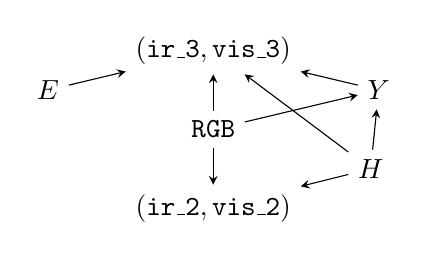
\begin{tikzpicture}[>=stealth, scale=1.0]
    \node (E) at (-2.1, 0.5) {$E$};
    \node (RGB) at (0, 0) {$\mathtt{RGB}$};
    \node (Y) at (2.1, 0.5) {$Y$};
    \node (H) at (2, -0.5) {$H$};
    \node (Bottom) at (0, -1) {$(\mathtt{ir\_2}, \mathtt{vis\_2})$};
    \node (Top) at (0, 1) {$\mathtt{(ir\_3, vis\_3)}$};

    \draw[->] (E) -- (Top);
    \draw[->] (RGB) -- (Top);
    \draw[->] (RGB) -- (Y);
    \draw[->] (Y) -- (Top);
    \draw[->] (RGB) -- (Bottom);
    \draw[->] (H) -- (Top);
    \draw[->] (H) -- (Bottom);
    \draw[->] (H) -- (Y);
\end{tikzpicture}